
% Journal Article
% LaTeX Template
% Version 1.4 (15/5/16)
%
% This template has been downloaded from:
% http://www.LaTeXTemplates.com
%
% Original author:
% Frits Wenneker (http://www.howtotex.com) with extensive modifications by
% Vel (vel@LaTeXTemplates.com)
%
% License:
% CC BY-NC-SA 3.0 (http://creativecommons.org/licenses/by-nc-sa/3.0/)
%
%%%%%%%%%%%%%%%%%%%%%%%%%%%%%%%%%%%%%%%%%

%----------------------------------------------------------------------------------------
%	PACKAGES AND OTHER DOCUMENT CONFIGURATIONS
%----------------------------------------------------------------------------------------

\documentclass[twoside,twocolumn]{article}

\usepackage{blindtext} % Package to generate dummy text throughout this template 

\usepackage[sc]{mathpazo} % Use the Palatino font
\usepackage[T1]{fontenc} % Use 8-bit encoding that has 256 glyphs
\linespread{1.05} % Line spacing - Palatino needs more space between lines
\usepackage{microtype} % Slightly tweak font spacing for aesthetics

\usepackage[english]{babel} % Language hyphenation and typographical rules

\usepackage[hmarginratio=1:1,top=32mm,columnsep=20pt]{geometry} % Document margins
\usepackage[hang, small,labelfont=bf,up,textfont=it,up]{caption} % Custom captions under/above floats in tables or figures
\usepackage{booktabs} % Horizontal rules in tables

\usepackage{lettrine} % The lettrine is the first enlarged letter at the beginning of the text

\usepackage{enumitem} % Customized lists
\setlist[itemize]{noitemsep} % Make itemize lists more compact

\usepackage{abstract} % Allows abstract customization
\renewcommand{\abstractnamefont}{\normalfont\bfseries} % Set the "Abstract" text to bold
\renewcommand{\abstracttextfont}{\normalfont\small\itshape} % Set the abstract itself to small italic text

\usepackage{titlesec} % Allows customization of titles
\renewcommand\thesection{\Roman{section}} % Roman numerals for the sections
\renewcommand\thesubsection{\roman{subsection}} % roman numerals for subsections
\titleformat{\section}[block]{\large\scshape\centering}{\thesection.}{1em}{} % Change the look of the section titles
\titleformat{\subsection}[block]{\large}{\thesubsection.}{1em}{} % Change the look of the section titles

\usepackage{fancyhdr} % Headers and footers
\pagestyle{fancy} % All pages have headers and footers
\fancyhead{} % Blank out the default header
\fancyfoot{} % Blank out the default footer
\fancyhead[C]{Image Colorization $\bullet$ Sep 2019} % Custom header text
\fancyfoot[RO,LE]{\thepage} % Custom footer text

\usepackage{titling} % Customizing the title section

\usepackage{hyperref} % For hyperlinks in the PDF

\usepackage{longtable}

\usepackage{graphicx}

\usepackage{amsmath,amssymb}

\DeclareRobustCommand{\bbone}{\text{\usefont{U}{bbold}{m}{n}1}}

\DeclareMathOperator{\EX}{\mathbb{E}}% expected value

\usepackage{multicol}


%----------------------------------------------------------------------------------------
%	TITLE SECTION
%----------------------------------------------------------------------------------------

\setlength{\droptitle}{-4\baselineskip} % Move the title up

\pretitle{\begin{center}\Huge\bfseries} % Article title formatting
\posttitle{\end{center}} % Article title closing formatting
\title{Image Colorization} % Article title
\author{%
\textsc{Tommaso Loss MATRICOLA} \\
\textsc{Matteo Marcuzzo 1207249}
 \\[1ex] % Your name
\normalsize University of Padua \\ % Your institution
%\normalsize \href{mailto:john@smith.com}{john@smith.com} % Your email address
%\and % Uncomment if 2 authors are required, duplicate these 4 lines if more
%\textsc{Jane Smith}\thanks{Corresponding author} \\[1ex] % Second author's name
%\normalsize University of Utah \\ % Second author's institution
%\normalsize \href{mailto:jane@smith.com}{jane@smith.com} % Second author's email address
}
\date{\today} % Leave empty to omit a date
\renewcommand{\maketitlehookd}{%
\begin{abstract}
\noindent
In this report we aim to cover some of the most recent advances in automatic image colorization of black and white pictures through the use of CNNs, as well as attempt to create our own implementation of one such. We describe the problem in its underconstrained nature, and discuss the approach by Zhang et al. \cite{Zhang:2016} which was used as our main reference. We then proceed to exhibit our implementation and the results we obtained. Lastly, we mention some different approaches and architectures that have surfaced in the most recent years, and make a comparison (MAYBE) (ANCHE NO SECONDO ME).
\end{abstract}
}

%----------------------------------------------------------------------------------------

\begin{document}

% Print the title
\maketitle

%----------------------------------------------------------------------------------------
%	ARTICLE CONTENTS
%----------------------------------------------------------------------------------------

\section{Introduction}

The task of colorizing grayscale images is not a simple one; to our imagination, some details might seem trivial (e.g. the sky is blue), yet some other are seemingly impossible to recover. As argued by Charpiat \cite{Charpiat:2008}, color prediction is, in fact, inherently multimodal - meaning many objects can take several plausible colorizations without a significant change in shape. To convince ourselves of this, it suffices to think a few examples. Apples, trees throughout seasons, artificial objects of various nature - a grayscale depiction of such has lost too much information for us to make a perfectly accurate guess. Nevertheless, we can easily imagine a plausible colorization, and would like an automatic system to be able to do the same.
Classical methods of the past have relied upon either user input or a large repository of reference images to use at test time. Recent approaches, however, have successfully leveraged the developments of deep convolutional neural networks (CNNs) to obtain a solution that requires no database and is fast at test time Larrson \cite{Larsson:2016}.\\
The first and key observation is that, in order to colorize images, a system must be able to interpret the semantic information of an image. In other words, it must be able to analyze the composition of the scene (what is in the picture) and where objects are located. Therefore, it comes as no surprise that CNNs are a perfect candidate for this task.\\
Furthermore, we may observe that colorization can be, in fact, seen as a classification problem where the classes to predict are a number of quantized color values (more on this later). Following Zhang’s \cite{Zhang:2016} implementation, we produced a system that predicts color probabilities over 313 quantized color bins. These probabilities are then used at the time of prediction to produce the final colorization. The prediction itself is produced by a single, feed forward pass through the network. \\
A last observation is that, usually, not all colors are represented equally in a picture. It’s easy for backgrounds to have a desaturated color that take up a large part of the picture (e.g. cloudy skies, walls, dirt); consequently, a network trained on a large set of images will be biased towards these colors. As suggested by Zhang \cite{Zhang:2016}, we introduce a form of class rebalancing in our loss function to produce brighter colors as well as push towards rarer ones.



%------------------------------------------------

\section{Approach}
In this section, we discuss the theoretical approach to the problem. This includes a discussion on the preferred color space used for the data, the formulation of an appropriate loss function, the class-rebalancing solution to desaturated colors, the network architecture itself and the way its results are interpreted.


\subsection{Color space}
Usual color spaces, as RGB or BGR, require the prediction of three different channels to recreate a colorized image. A common approach is to instead adopt the CIE-Lab color space, which proves to be useful in that it restricts the problem by one dimension. This color space is also comprised of three channels, but has the useful characteristic that all grayscale information is stored in one of such. Indeed, the first channel (namely \textbf{L}) tracks the “lightness” value of a pixel (ranging from 0 for black to 100 for white). Channel \textbf{A} represent instead the color range between red and green, while channel \textbf{B} does the same for blue and yellow. As said, adopting this image representation technique makes it fairly trivial to obtain the black and white version of a picture as the problem input (by simply discarding the \textbf{A} and \textbf{B} channels). Furthermore, it simplifies the classification task, as there are only two channels to predict over.

\subsection{Loss function}
As was briefly previewed, our system is in fact a classification model which returns probabilities over a set of color classes. One of the most commonly used loss functions in multinomial classification problems is that of \texttt{Cross Entropy}, which calculates the average difference between the ground truth and the predicted probability distribution. 
In order to perform classification, however, we first have to define the classes we want to predict. To do this, we synthesize the color space into a small number of AB pairs (with \textbf{L} = 50). A grid with space size 10 is overlaid onto the color space, thus reducing the number of relevant color pairs by a factor of ten. From the remaining colors, out of gamut ones are removed to obtain the final 313 color classes used in the classification task.

In order to make a comparison, however, we now require ground truth values in the same form of the predicted probabilities. The real color values are therefore transformed into probability distributions. This is achieved through soft-encoding, by mapping each pixel color to its nearest five quantized AB color pairs and giving each one a weight based on the euclidean distance from the original color. Such distance-weights are then smoothed with a Gaussian kernel (with =5). [[ref 31 del paper]]

\begin{equation}
L_{cl}(P,T) = - \sum_{q} \: T_q \: log(P_q)
\end{equation}

However, that alone is not enough to obtain a meaningful colorization. This is because of the inherently uneven color distribution; in particular, background and foreground colors such as blue and green are much more prevalent than rare colors like purple. The resulting model will therefore be biased to more common colors, neglecting rare ones. 
The solution to this problem proposed by Zhang \cite{Zhang:2016} is to reweight the probabilities by a factor based on the scarcity of the color. This process, named class-rebalancing, allows us to obtain our final loss formulation:

\begin{equation}
L_{cl}(P,T) = - \sum_{h,w}(v(T_{h,w}) \: \sum_{q} \: T_{h,w,q} \: log(P_{h,w,q}))
\end{equation}

\subsection{Class-rebalancing}

The idea of class-rebalancing is to take into account the inherent imbalance of class representation by reweighting the loss of each pixel at train time based on the pixel color rarity \cite{Zhang:2016}. The computation of color weights starts by calculating the number of occurrences of each AB color pair over the whole image dataset (mapping each pixel to the closest bin). The resulting color frequency values are then turned into probability distributions, which are smoothed with a gaussian kernel as is done with ground truth probabilities ($\sigma$ = 5). In order to lower the significant impact of these weights, these are mixed with a uniform probability distribution (p = 1/313). Finally, we take the reciprocal of the result in order to reverse the probability values, as we would like frequent colors to have little weights and vice-versa. The mixing factor suggested by Zhang \cite{Zhang:2016} is of $1/2$. Furthermore, the result is normalized again, so that the weighting factor is 1 on expectation.


\begin{equation}
w = (1 - \lambda)p + \frac{\lambda}{U})^{-1}
\end{equation}


\subsection{Network architecture}

The network architecture follows the one proposed by Zhang \cite{Zhang:2016}, Table \ref{tab:network}. The network itself is comprised of 30 layers, which are either 2D convolutional layers or batch normalization layers.


\subsubsection{Layers}
The network is divided into 8 layer blocks, all of which are followed by a batch normalization layer (except for the last one, where a 1x1 conv and cross-entropy layer is imposed). The following table describes the layers and their parameter values.


\begin{table*}[t]
\centering
\captionof{table}{Network structure}
\label{tab:network}
\begin{tabular}{|c|c|c|c|c|c|}
	\hline
	\hline
	Layer & Filters & Spac. Res. & Kernel size & Stride & Dilation\\ 
	\hline
	\hline
	\multicolumn{6}{|c|}{input data (with size e.g. 224 * 224)}\\ \hline
	conv1\_1 & 64 & 224 & 3x3 & (1,1) & 1 \\ \hline
	conv1\_2 & 64 & 112 & 3x3 & (2,2) & 1 \\ \hline
	\multicolumn{6}{|c|}{Batch normalization}\\ \hline
	conv2\_1 & 128 & 112 & 3x3 & (1,1) & 1 \\ \hline
	conv2\_2 & 128 & 56 & 3x3 & (2,2) & 1 \\ \hline
	\multicolumn{6}{|c|}{Batch Normalization}\\ \hline
	conv3\_1 & 256 & 56 & 3x3 & (1,1) & 1 \\ \hline
	conv3\_2 & 256 & 56 & 3x3 & (1,1) & 1 \\ \hline
	conv3\_3 & 256 & 28 & 3x3 & (2,2) & 1 \\ \hline
	\multicolumn{6}{|c|}{Batch normalization}\\ \hline
	conv4\_1 & 512 & 28 & 3x3 & (1,1) & 1 \\ \hline
	conv4\_2 & 512 & 28 & 3x3 & (1,1) & 1 \\ \hline
	conv4\_3 & 512 & 28 & 3x3 & (1,1) & 1 \\ \hline
	\multicolumn{6}{|c|}{Batch normalization}\\ \hline
	conv5\_1 & 512 & 28 & 3x3 & (1,1) & 2 \\ \hline
	conv5\_2 & 512 & 28 & 3x3 & (1,1) & 2 \\ \hline
	conv5\_3 & 512 & 28 & 3x3 & (1,1) & 2 \\ \hline
	\multicolumn{6}{|c|}{Batch normalization}\\ \hline
	conv6\_1 & 512 & 28 & 3x3 & (1,1) & 2 \\ \hline
	conv6\_2 & 512 & 28 & 3x3 & (1,1) & 2 \\ \hline
	conv6\_3 & 512 & 28 & 3x3 & (1,1) & 2 \\ \hline
	\multicolumn{6}{|c|}{Batch normalization}\\ \hline
	conv7\_1 & 256 & 28 & 3x3 & (1,1) & 1 \\ \hline
	conv7\_2 & 256 & 28 & 3x3 & (1,1) & 1 \\ \hline
	conv7\_3 & 256 & 28 & 3x3 & (1,1) & 1 \\ \hline
	\multicolumn{6}{|c|}{Batch normalization}\\ \hline
	\multicolumn{6}{|c|}{2D Upsampling with size 2*2}\\ \hline
	conv8\_1 & 128 & 56 & 3x3 & (0.5,0.5)\footnote{The .5 stride is simulated through the 2d upsampling. Earlier implementations made instead use of a deconvolutional layer, but we found this other approach to work better in practice.
	}. & 1 \\ \hline
	conv8\_2 & 128 & 56 & 3x3 & (1,1) & 1 \\ \hline
	conv8\_3 & 128 & 56 & 3x3 & (1,1) & 1 \\ \hline
	\multicolumn{6}{|c|}{Softmax Layer}\\ \hline
	
\end{tabular}
\end{table*}

\subsection{Parameters}

\begin{equation}
Var(w_i) = \frac{2}{fan\_in}
\end{equation}

\begin{equation}
Loss = Error(y,\tilde{y}) + \lambda\sum_{i=1}^{N} w_i^2
\end{equation}


\subsection{Prediction evaluation}

Once the model has been trained, prediction is done through a single, feed forward pass through the network, which accepts the L channel of a picture and produces a probability distribution over the 313 quantized colors for each pixel.

It remains to decide how to use this information to produce our colorization. One choice is to take the most frequent and probable values; while this idea results very vibrant colors, it often produces spatially inconsistent results and “hard transitions” from one color to the other. A better approach could therefore be to take the mean over each of the quantized bins, weighing them by their probability. This ensures softer transitions, but runs into the unwanted consequence that colors become desaturated, as too much importance is attributed to lower probability colors.

The solution proposed by Zhang \cite{Zhang:2016} attempts to have the best of both worlds. The authors suggest taking what they name “annealed mean” of the distribution. This consists of an interpolation of the softmax distribution by means of a temperature value T, and consequently taking the mean of the result. Strictly speaking, this translates into dividing each value by the aforementioned temperature value, which ranges from 0 to 1 (the suggested value is 0.38, which we adhered to). This ensures that more importance is given to high probability values, resulting into the vibrant colorization desired as well as better spatial consistency. 

\begin{equation}
H(P) = \EX[f(P)] 
\end{equation}

\begin{equation}
f(P) = \frac{\exp(log(P)/T)}{\sum_q \: \exp(log(P_q)/T)}
\end{equation}

Text requiring further explanation\footnote{Example footnote}.

%------------------------------------------------


\section{Experimentation}

\subsection{Implementation}

In this section, we briefly discuss the actual implementation and the results of our experiments. This includes a discussion on libraries and data used, hardware specifics and graph.

\subsection{Dataset}

\begin{figure}
	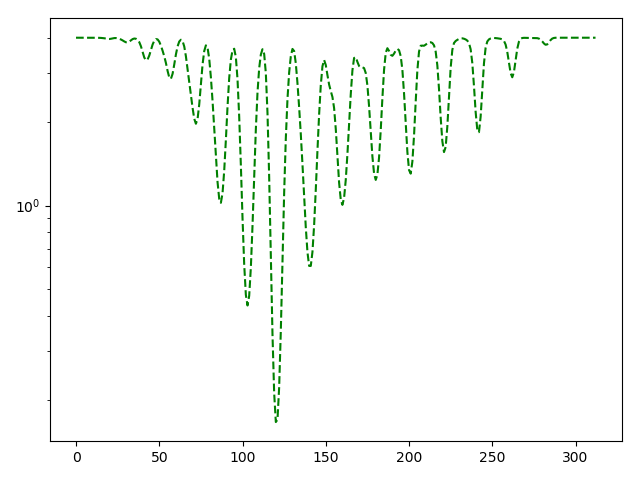
\includegraphics[width=\linewidth]{img/ours.png}
	\caption{Ours color prior results}
	\label{fig:oursprior}
\end{figure}

\begin{figure}
	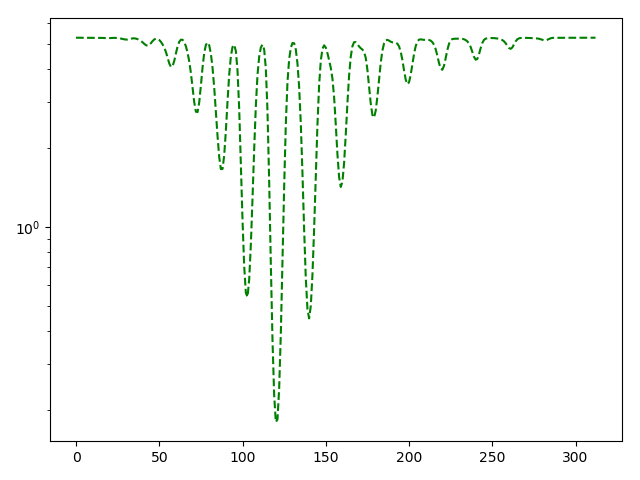
\includegraphics[width=\linewidth]{img/zhang.png}
	\caption{Zhang \cite{Zhang:2016} color prior results}
	\label{fig:zhangprior}
\end{figure}

\subsection{Metrics}

\subsection{Hyperparameters}

\subsection{Hardware details}

\subsection{Performance and results}

\begin{figure}
	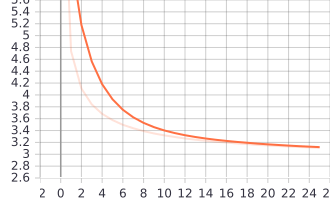
\includegraphics[width=\linewidth]{img/loss.png}
	\caption{Loss}
	\label{fig:loss}
\end{figure}

\begin{figure}
	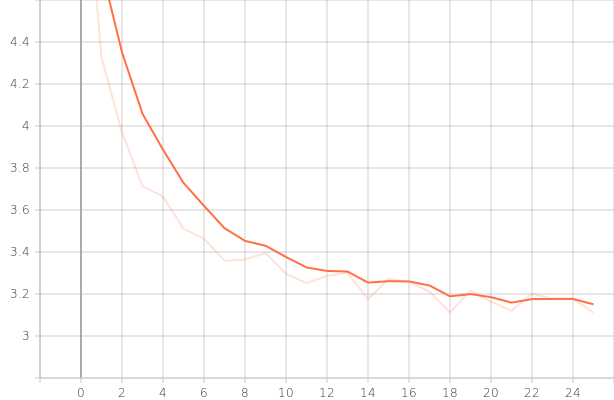
\includegraphics[width=\linewidth]{img/val_loss.png}
	\caption{Validation Loss}
	\label{fig:valloss}
\end{figure}

%------------------------------------------------

\section{Considerations}

\subsection{Recent developments}

%------------------------------------------------

%------------------------------------------------

\section{Conclusions}

%------------------------------------------------

%----------------------------------------------------------------------------------------
%	REFERENCE LIST
%----------------------------------------------------------------------------------------

\begin{thebibliography}{99} % Bibliography - this is intentionally simple in this template

\bibitem[1]{Zhang:2016}
Richard Zhang, Phillip Isola, Alexei A. Efros (2016).
\newblock Colorful Image Colorization.
 
\bibitem[2]{Charpiat:2008}
Charpiat, G., Hofmann, M., Scholkopf, B. (2008).
\newblock Automatic image colorization via multimodal
predictions.
\newblock Computer Vision-ECCV 2008. Springer 126 - 139

\bibitem[3]{Larsson:2016}
Larsson, G., Maire, M., Shakhnarovich, G. (2016).
\newblock Learning representations for automatic
colorization.
\newblock European Conference on Computer Vision (2016)

\bibitem[1]{Zhang:2016}
Richard Zhang, Phillip Isola, Alexei A. Efros (2016).
\newblock Colorful Image Colorization.

\bibitem[1]{Zhang:2016}
Richard Zhang, Phillip Isola, Alexei A. Efros (2016).
\newblock Colorful Image Colorization.

\bibitem[1]{Zhang:2016}
Richard Zhang, Phillip Isola, Alexei A. Efros (2016).
\newblock Colorful Image Colorization.

\end{thebibliography}

%----------------------------------------------------------------------------------------

\end{document}
